\documentclass[12pt,a4paper,openany,fleqn]{book}

\usepackage{cmap}
\usepackage[left=1.3cm, right=1.3cm, top=1.4cm, bottom=1.3cm]{geometry}
\usepackage[utf8]{inputenc}
\usepackage[english, russian]{babel}
\usepackage{indentfirst}
\usepackage{amsmath}
\usepackage{amssymb}
\usepackage{amsthm}
\usepackage{gensymb}
\usepackage{mathrsfs}
\usepackage{bm}
\usepackage{perpage}
\usepackage{enumitem}
\usepackage[unicode, colorlinks=true]{hyperref}
\usepackage{tikz}
\usepackage{tabularx}
\usepackage{graphicx}
\usepackage{xfrac}



\setcounter{tocdepth}{1}

\setlength{\mathindent}{0em}

\addto{\captionsrussian}{\renewcommand{\contentsname}{Содержание}}
\addto{\captionsrussian}{\renewcommand{\chaptername}{Лекция}}

\newcommand {\defeq}{\stackrel{\hspace{0.09 cm}de\!f}{=}}
\newcommand {\eqdef}{\defeq}
\newcommand{\iffdef}{\stackrel{\hspace{0.09 cm}de\!f}{\iff}}
\newcommand{\R}{\ensuremath{\mathbb{R}}}
\newcommand{\Cf}{\ensuremath{\mathcal{C}}}
\newcommand{\J}{\ensuremath{\mathcal{J}}}
\newcommand{\mc}[1]{\ensuremath{\mathcal{#1}}}
\newcommand{\Cfn}[2][]{\ensuremath{\Cf{\mathstrut}^{#2}_{#1}}}
\newcommand{\der}[2]{\ensuremath{\frac{d#1}{d#2}}}
\newcommand{\dder}[2]{\ensuremath{\frac{d^2#1}{d#2^2}}}
\newcommand{\pder}[2]{\ensuremath{\frac{\partial#1}{\partial#2}}}
\newcommand{\pdder}[2]{\ensuremath{\frac{\partial^2#1}{\partial#2^2}}}
\newcommand{\eps}{\varepsilon}
\newcommand{\K}{\mc{K}}
\newcommand{\LL}{\ensuremath{L}}
\newcommand{\fL}[1][{[a,b]}]{\ensuremath{\mathscr{L}\hspace*{-0.11 cm}{\mathstrut}_{2}\scriptstyle#1}}
\newcommand{\norm}[1]{\ensuremath{\left\|#1\right\|}}
\newcommand{\Ul}[1][\lambda]{\ensuremath{\mc{U}\!{\mathstrut}_{#1}}}

\DeclareMathOperator\Tg{tg}


\pagestyle{headings}

\theoremstyle{definition}
\newtheorem{_def}{Определение}[section]
\newtheorem{_lemm}{Лемма}[section]
\newtheorem{_teor}{Теорема}[section]
\newtheorem*{_rem}{Замечание}
\newtheorem*{_con}{Следствие}
\MakePerPage{footnote}

\setlist[enumerate,1]{label=\alph*), ref=\alph*)}

\newlist{enumerate1}{enumerate}{1}
\setlist[enumerate1,1]{label=\arabic*), ref=\arabic*)}
\newlist{enumerateA}{enumerate}{1}
\setlist[enumerateA,1]{label=\Alph*), ref=\Alph*)}

\newlist{enumerateD}{enumerate}{2}
\setlist[enumerateD,1]{label=\arabic*., ref=\arabic*.}
\setlist[enumerateD,2]{{label=\alph*., ref=\alph*.}}

\newlist{enumerateBr}{enumerate}{1}
\setlist[enumerateBr,1]{label=\underline{(\arabic*)}, ref=\underline{(\arabic*)}}
\begin{document}
	\author{Г.\,М.~Жислин}
	\title{Лекции по вариационному исчислению и уравнениям математической физики}
	\date{Конспектировал А.\,Г.~Чубаров}
	
	
	
	\maketitle
	
	
	\renewcommand{\thepart}{\Asbuk{part}}
	\renewcommand{\thechapter}{\arabic{chapter}}
	\renewcommand{\thesection}{\arabic{section}}
	\renewcommand{\thesubsection}{\Roman{subsection}}
	\renewcommand{\thefootnote}{\roman{footnote}}
	\renewcommand{\phi}{\varphi}
	\renewcommand{\Re}{\ensuremath{\mc{R}e\,}}
	\renewcommand{\Im}{\ensuremath{\mc{I}m\,}}
	\numberwithin{equation}{section}
	
	\setcounter{chapter}{6}
	\chapter{}
	\label{lecture7}
	\section{Оператор Штурма с другими граничными условиями.}
	\label{lecture7section1}
	В физических задачах, которые приводят к нахождению собственных значений оператора Штурма кроме граничных условий $y(a)=y(b)=0$ встречаются и другие типы граничных условий\footnote[1]{Мы увидим это в части <<Уравнения математической физики>>.}. Поэтому возникает необходимость в изучении подобных задач.
	
	Общий вид граничных условий:
	\begin{equation*}
		\begin{cases}
			\alpha_1\cdot y'(a)+\alpha_2\cdot y(a)=0,\\
			\beta_1\cdot y'(b)+\beta_2\cdot y(b)=0,
		\end{cases}
	\end{equation*} 
	где $\alpha_j,\,\beta_j$ --- фиксированные числа. Если $\alpha_1=0$ (или $\beta_1=0$), то тогда граничные условия переходят соответственно в
	\begin{equation*}
		\hfill\alpha_2\cdot y(a)=0\quad\Rightarrow\quad y(a)=0\qquad(\text{или в }\beta_2\cdot y(b)=0\quad\Rightarrow\quad y(b)=0).\hfill
	\end{equation*}  
	Поэтому мы будем считать $\alpha_1\neq0$, $\beta_1\neq0$. Тогда поделив на $\alpha_1$ и $\beta_1$ мы получим
	\begin{equation*}
		\hfill y'(a)=-\frac{\alpha_2}{\alpha_1}\cdot y(a),\quad y'(b)=-\frac{\beta_2}{\beta_1}\cdot y(b).\hfill
	\end{equation*}
	Положим $\gamma_1\eqdef-\alpha_2/\alpha_1$, $\gamma_2\eqdef\beta_2/\beta_1$. В физических задачах $\gamma_1\,\gamma_2\geqslant0$. Таким образом мы будем рассматривать граничные условия 
	\begin{equation}
		\label{l6:eq:1}
		\hfill y'(a)=\gamma_1\cdot y(a),\  y'(b)=-\gamma_2\cdot y(b),\quad\gamma_1,\,\gamma_2\geqslant0.\hfill
	\end{equation} 
	Таким образом в качестве области определения оператора Штурма 
	\begin{equation*}
		\hfill Ly=-\der{}{x}\Big(Q\cdot y'\Big)+P\cdot y\hfill
	\end{equation*}
	мы возьмём область
	\begin{equation*}
		\hfill\mc{D}_{L}^0\eqdef\left\{y(x)|y\in\Cfn[{[a,b]}]{2},\ y'(a)=\gamma_1\cdot y(a),\ y'(b)=-\gamma_2\cdot y(b),\ \gamma_1,\,\gamma_2\geqslant0\right\}_{\displaystyle.}\hfill
	\end{equation*}
	Как и при изучении оператора $L$ в $\mc{D}_L$\footnote{\vspace*{-0,4cm}\begin{equation*}
			\qquad\mc{D}_L=\left\{y(x)|y\in\Cfn[{[a,b]}]{2},\ y(a)=y(b)=0\right\}_{\displaystyle.}
	\end{equation*}}, мы в первую очередь рассмотрим оператор $L$ в $\mc{D}_{L}^0$ с постоянными коэффициентами $Q(x)=C_1$, $P(x)=C_2$, $[a,b]=[0,l]$. Как и раньше считаем $C_1>0$, что касается отрезка $[0,l]$, то мы можем перейти к нему от произвольного отрезка $[a,b]$ заменой переменной: $x'=x-a$. Тогда $x'\in[0,l]$, где $l=b-a$. Чтобы не загромождать изложение мы штрих писать не будем.

	Итак, рассматриваем задачу на нахождение собственных значений и собственных функций оператора 
	\begin{equation}
		\label{l7:eq:2}
		\hfill L y=-C_1\cdot y''+C_2\cdot y=\lambda\cdot y,\quad y\in\mc{D}_L^0.\hfill
	\end{equation}
	Переносим $\lambda\cdot y$ в левую часть~\eqref{l7:eq:2} и делим на $-C_1$. Получаем
	\begin{equation}
		\label{l7:eq:3}
		\hfill y''+\frac{\lambda-C_2}{C_1}\cdot y=0.\hfill
	\end{equation} 
	Положим $\omega^2\eqdef\displaystyle\frac{\lambda-C_2}{C_1}$ и попытаемся доказать, что $\omega^2$ --- вещественно и определить знак $\omega^2$ (мы пока не знаем, что $\omega^2$ --- вещественно). Умножим обе части~\eqref{l7:eq:3} на $y$ скалярно. Получим
	\begin{equation}
		\label{l7:eq:4}
		\hfill\int\limits_0^l y''\cdot\overline{y}\,dx+\omega^2\cdot\int\limits_0^l|y|^2\,dx=0.\hfill
	\end{equation}
	Далее
	\begin{multline*}
		\int\limits_0^l\underbrace{\overline{y}}_{v}\cdot \underbrace{y''\,dx}_{du}=y'\cdot\overline{y}\mathop{\Big|}\limits_0^l-\int\limits_0^l|y'|^2\,dx=y'(l)\cdot \overline{y}(l)-y'(0)\cdot\overline{y}(0)-\int\limits_0^l|y'|^2\,dx=\left|\parbox{0.14\textwidth}{\centering в силу граничных условий}\right|=\\
		=-\gamma_2\cdot|y(l)|^2-\gamma_1\cdot|y(0)|^2-\int\limits_0^l|y'(x)|^2\,dx.
	\end{multline*}
	Подставляя в~\eqref{l7:eq:4}, имеем 
	\begin{equation}
		\label{l7:eq:5}
		\hfill-\gamma_2\cdot|y(l)|^2-\gamma_1\cdot|y(0)|^2-\int\limits_0^l|y'(x)|^2\,dx+\omega^2\cdot\int\limits_0^l|y|^2\,dx=0.\hfill
	\end{equation}
	Отсюда следует, что $\omega^2$ --- вещественно и $\omega^2\geqslant0$. Посмотрим, возможно ли равенство $\omega^2=0$. При $\omega^2=0$ из~\eqref{l7:eq:5} следует, что 
	\begin{equation*}
		\hfill\int\limits_0^l|y'(x)|^2\,dx=0\quad\Rightarrow\quad y(x)=const.\hfill
	\end{equation*}  
	В этом случае $y(0)\neq0$, $y(l)\neq0$ (иначе $y(x)\equiv0$). Поэтому из~\eqref{l7:eq:5} видим, что $\omega^2=0$ может быть при $\gamma_1=0$, $\gamma_2=0$. Функция $y(x)=const$ в этом случае удовлетворяет уравнению~\eqref{l7:eq:3} с $\omega^2=0$ и граничным условиям $y'(0)=y'(l)=0$. Если мы нормируем $y(x)$, то получим $y=1\!\!\bigm/\!\!\sqrt{l}$. Далее будем считать $\omega^2>0$. Итак, решаем уравнение~\eqref{l7:eq:3}
	\begin{equation}
		\label{l7:eq:6}
		\hfill y''+\omega^2\cdot y=0.\hfill
	\end{equation}
	Общее решение
	\begin{equation*}
		\hfill y=d_1\cdot\sin(\omega\cdot x)+d_2\cdot\cos(\omega\cdot x).\hfill
	\end{equation*}
	Находим $y'(0)$, $y'(l)$ и записываем граничные условия 
	\begin{equation*}
		\hfill y'(0)=\gamma_1\cdot y(0),\quad y'(l)=-\gamma_2\cdot y(l).\hfill
	\end{equation*}
	$y'(x)=\omega\cdot d_1\cdot\cos(\omega\cdot x)-\omega\cdot d_2\cdot\sin(\omega\cdot x)$, поэтому
	\begin{equation}
		\label{l7:eq:7}
		\begin{cases}
			\omega\cdot d_1=\gamma_1\cdot d_2,\\
			d_1\cdot\omega\cdot\cos(\omega\cdot l)-d_2\cdot\omega\cdot\sin(\omega\cdot l)=-d_1\cdot\gamma_2\cdot\sin(\omega\cdot l)-d_2\cdot\gamma_2\cdot\cos(\omega\cdot l).
		\end{cases}
	\end{equation}
	Получили систему двух однородных линейных уравнений с двумя неизвестными: $d_1,\,d_2$. Для существования не нулевого решения определитель системы должен равняться нулю.\footnote{Конечно, можно из первого уравнения выразить $d_1$ через $d_2$, или $d_2$ через $d_1$ и подставить во второе уравнение. Ошибки не будет. Однако стандартный способ решения (приравнивание определителя к нулю) лучше и надо приучаться к нему.} Выпишем определитель системы~\eqref{l7:eq:7}
	\begin{gather}
		\begin{vmatrix}
			\omega&-\gamma_1\\
			\omega\cdot\cos(\omega\cdot l)+\gamma_2\cdot\sin(\omega\cdot l)&\gamma_2\cdot\cos(\omega\cdot l)-\omega\cdot\sin(\omega\cdot l)
		\end{vmatrix}=0,\notag
		\intertext{то есть}\omega\cdot\gamma_2\cdot\cos(\omega\cdot l)-\omega^2\cdot\sin(\omega\cdot l)+\gamma_1\cdot\omega\cdot\cos(\omega\cdot l)+\gamma_1\cdot\gamma_2\cdot\sin(\omega\cdot l)=0.
		\label{l7:eq:8}
	\end{gather}
	Если $\cos(\omega\cdot l)=0$, то $\sin(\omega\cdot l)\neq0$ и сокращая в~\eqref{l7:eq:8} на $sin(\omega\cdot l)$ (после зануления $\cos(\omega\cdot l)$) мы получим 
	\begin{equation*}
		\hfill-\omega^2+\gamma_1\cdot\gamma_2,\quad\omega=\sqrt{\gamma_1\cdot\gamma_2},\hfill
	\end{equation*}
	но так как $\cos(\omega\cdot l)=0$, то $l\cdot\omega_k=\displaystyle\frac{\pi}{2}+\pi\cdot k$. Таким образом этот случай имеет место, если для какого-то $k$ ($k=0,1,2,\ldots$)
	\begin{equation}
		\label{l7:eq:9}
		\hfill\frac{\pi}{2}+\pi\cdot k=\sqrt{\gamma_1\cdot\gamma_2}\cdot l,\hfill
	\end{equation} 
	то есть число $(l\cdot\sqrt{\gamma_1\cdot\gamma_2}-\pi/2)\bigm/\pi$ --- целое, то мы получаем из равенства $\omega=\sqrt{\gamma_1\cdot\gamma_2}$ собственное значение 
	\begin{equation*}
		\hfill\frac{\lambda-C_2}{C_1}=\gamma_1\cdot\gamma_2\quad\Rightarrow\quad\lambda_0=C_1\cdot\gamma_1\cdot\gamma_2+C_2\hfill
	\end{equation*}
	и затем из первого уравнения системы~\eqref{l7:eq:7} найдём $d_2=d_1\cdot\sqrt{\gamma_2\bigm/\gamma_1}$, подставляем в решение уравнения~\eqref{l7:eq:6} и получаем 
	\begin{equation*}
		\hfill y_0=d_1\cdot\left(\sin(\omega\cdot x)+\sqrt{\frac{\gamma_2}{\gamma_1}}\cdot\cos(\omega\cdot x)\right)\hfill
	\end{equation*}
	Это и есть собственная функция, отвечающая собственному значению $\lambda_0$ при выполнении~\eqref{l7:eq:9} для какого-то целого $k$. 
	
	Далее считаем $\cos(\omega\cdot l)\neq0$. Перенесём в выражении определителя~\eqref{l7:eq:8} члены с $\sin(\omega\cdot l)$ в правую часть равенства, получим
	\addtocounter{equation}{1}
	\begin{equation}
		\label{l7:eq:10c}
		\omega\cdot\cos(\omega\cdot l)\cdot(\gamma_1+\gamma_2)=\omega^2\cdot\sin(\omega\cdot l)-\gamma_1\cdot\gamma_2\cdot\sin(\omega\cdot l)=(\omega^2-\gamma_1\cdot\gamma_2)\cdot\sin(\omega\cdot l),\tag{\theequation c}
	\end{equation}
	где $\cos(\omega\cdot l)\neq0$ и $\omega^2-\gamma_1\cdot\gamma_2\neq0$\footnote{Если бы $\omega^2-\gamma_1\cdot\gamma_2=0$, то в силу~\eqref{l7:eq:10c} $\cos(\omega\cdot l)\cdot(\gamma_1+\gamma_2)=0$, но $\cos(\omega\cdot l)\neq0$, значит $\gamma_1=\gamma_2=0$. Но тогда $\omega=0$, а этот случай нами уже рассмотрен. Следовательно мы можем считать $\omega\neq0$ и значит $\omega^2-\gamma_1\cdot\gamma_2\neq0$.}. После деления~\eqref{l7:eq:10c} на $\cos(\omega\cdot l)$ имеем 
	\begin{equation}
		\label{l7:eq:10a}
		\hfill\omega\cdot(\gamma_1+\gamma_2)=(\omega^2-\gamma_1\cdot\gamma_2)\Tg(\omega\cdot l),\tag{\theequation a}\hfill
	\end{equation} 
	откуда 
	\begin{equation}
		\label{l7:eq:10b}
		\hfill\Tg(\omega\cdot l)=\frac{\omega\cdot(\gamma_1+\gamma_2)}{\omega^2-\gamma_1\cdot\gamma_2}\quad\text{или}\quad\Tg(\omega\cdot l)=\cfrac{\gamma_1+\gamma_2}{\omega-\cfrac{\gamma_1\cdot\gamma_2}{\omega}}.\hfill\tag{\theequation b}
	\end{equation}
	Удобно положить $z=l\cdot\omega$, тогда уравнение~\eqref{l7:eq:10b} запишется в виде
	\begin{equation}
		\label{l7:eq:11}
		\hfill\Tg(z)=\cfrac{(\gamma_1+\gamma_2)\cdot l}{z-\cfrac{\gamma_1\cdot\gamma_2\cdot l^2}{z}}.\hfill
	\end{equation}
	Это и есть уравнение для нахождения $z$, а значит $\omega$ и $\lambda$.
	
	Рассмотрим в уравнении~\eqref{l7:eq:11} сначала частный случай, когда~\eqref{l7:eq:11} можно решить в явном виде. Пусть $\gamma_1=\gamma_2=0$, то есть граничные условия $y'(0)=0$, $y'(l)=0$. В этом случае решения уравнения~\eqref{l7:eq:11} получаем из условия
	\begin{equation*}
		\hfill\Tg(z)=0\quad\Rightarrow\quad\sin(z)=0\quad\Rightarrow\quad z=\omega\cdot l=\pi\cdot k,\ k=1,2,\ldots\footnotemark{}\hfill
	\end{equation*} \footnotetext{$k=0$ --- рассматриввали раньше.}Откуда
	\begin{equation*}
		\hfill\omega_k=\frac{\pi\cdot k}{l}\quad\Rightarrow\quad\frac{\lambda_k-C_2}{C_1}=\left(\frac{\pi\cdot k}{l}\right)^2\quad\Rightarrow\quad\lambda_k=C_1\cdot\left(\frac{\pi\cdot k}{l}\right)^2+C_2.\hfill
	\end{equation*}
	Собственная функция $y_k$ есть
	\begin{equation*}
		\hfill y_k=d_{1k}\cdot\sin(\omega_k\cdot x)+d_{2k}\cdot\cos(\omega_k\cdot x),\hfill
	\end{equation*}
	где связь между $d_{1k}$ и $d_{2k}$ даётся первым уравнением системы~\eqref{l7:eq:6}
	\begin{equation*}
		\hfill\omega_k\cdot d_{1k}=\gamma_1\cdot d_{2k}\quad\Rightarrow\quad d_{1k}=0,\text{а }d_{2k}\text{ --- произвольное число.}\hfill
	\end{equation*}
	Таким образом 
	\begin{equation*}
		\hfill y_k=d_{2k}\cdot\cos\left(\frac{\pi\cdot k}{l}\right),\hfill
	\end{equation*}
	где $d_{2k}$ выбирается из условия $\norm{y_k}=1$.
	
	Возвращаемся к решаемому уравнению~\eqref{l7:eq:11} и обозначим его правую часть через $\Psi(z)$:
	\begin{equation}
		\label{l7:eq:11a}
		\hfill\Tg(z)=\Psi(z),\hfill\tag{\theequation a}
	\end{equation}	
	где $\Psi(z)=\dfrac{(\gamma_1+\gamma_2)\cdot l}{z-\dfrac{\gamma_1\cdot\gamma_2\cdot l^2}{z}}$.
	
	\noindent При $\gamma_1+\gamma_2>0$ (а мы рассматриваем именно этот случай) мы не можем найти аналитически решения уравнения~\eqref{l7:eq:11a} и вынуждены искать их графически. Для этого на плоскости $y,\,z$ построим графики функций $y_1=\Tg(z)$, $y_2=\Psi(z)$ и  <<абсциссы>> (то есть точки $z_k$) отвечающие точкам пересечения графиков и дадут решения~\eqref{l7:eq:11a}. Рассмотрим сначала случай, когда одно (только одно!) из чисел $\gamma_1,\,\gamma_2$ равно нулю. Пусть для определённости $\gamma_2=0$. Уравнение~\eqref{l7:eq:11a} примет вид
	\begin{equation*}
		\hfill\Tg(z)=\dfrac{\gamma_1\cdot l}{z}.\hfill
	\end{equation*}
	\begin{center}
		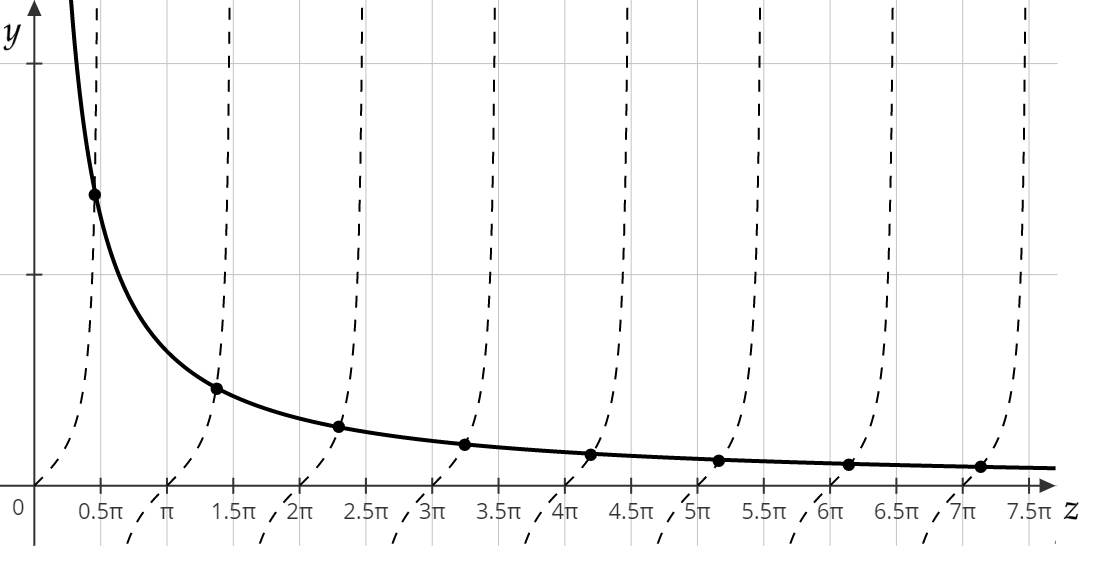
\includegraphics[width=0.7\linewidth]{picture1}
	\end{center}
	Рисуем графики мы видим, что точки пересечения графиков отвечают всё меньшим значениям $\Tg(z)$, то есть стремятся к $\pi\cdot k$, то есть очевидно, что $|z_k-\pi\cdot  k|\to0$, при $k\to\infty$. Откуда
	\begin{equation*}
		\hfill z_k^2=l^2\cdot\omega_k^2=\dfrac{l^2\cdot(\lambda_k-C_2)}{C_1}\geqslant C_0\cdot k^2,\hfill
	\end{equation*}	
	где $C_0>0$ некоторая константа. Отсюда
	\begin{equation*}
		\hfill\lambda_k\geqslant\frac{C_0\cdot C_1}{l^2}\cdot k^2+C_2.\hfill
	\end{equation*}
	Значит, собственные значения растут со скоростью $k^2$.
	
	Рассмотрим наконец общий случай $\gamma_1\cdot\gamma_2>0$. В этом случае функция $\Psi(z)$ имеет разрыв при $z=z_0=l\cdot\sqrt{\gamma_1\cdot\gamma_2}$, и $\Psi(z_0+0)=+\infty$, $\Psi(z_0-0)=-\infty$.
	\begin{center}
		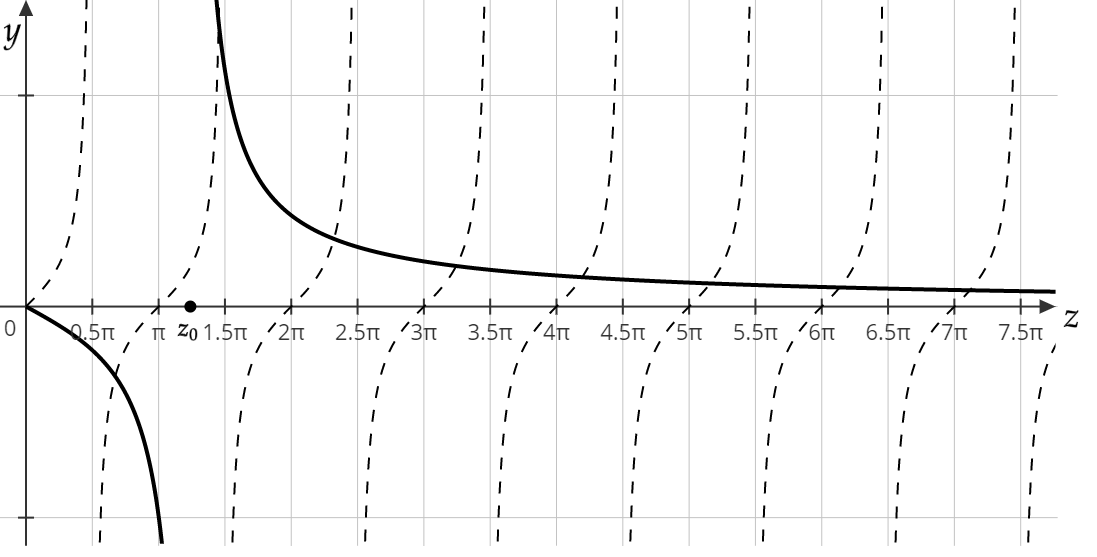
\includegraphics[width=0.7\linewidth]{picture2}
	\end{center}
	На чертеже $\pi<z_0<\frac{3}{2}\cdot\pi$. Мы видим, что появилась новая точка пересечения на графике $\Psi(z)$ и $\Tg(z)$. В зависимости от положения $z_0$ таких точек или нет --- если $z_0\leqslant{\pi}/{2}$ --- или несколько при $z>{\pi}/{2}$. Пусть слева от $z_0$ имеется $m_0$ решений уравнения~\eqref{l7:eq:11a}, $m_0\geqslant0$ и число $m_1$ таково, что $\pi\cdot m_1\leqslant z_0\leqslant\pi\cdot(m_1+1)$, $m_1\geqslant0$ (связь $m_0$ и $m_1$ нам не интересна). Тогда из графиков $\Tg(z)$ и $\Psi(z)$ видно, что решения $z_{m_0+k}$ будут асимптотически стремиться к $(m_1+k)\cdot\pi$, то есть
	\begin{equation*}
		\hfill\displaystyle z_{m_0+k}-\pi\cdot(m_1+k)\to0,\hfill
	\end{equation*}
	откуда полагая $s=m_0+k$ получаем 
	\begin{equation*}
		\hfill z_s-\pi\cdot(m_1-m_0+s)\to0\quad\text{при}\quad s\to\infty\hfill
	\end{equation*}
	и, значит, 
	\begin{equation*}
		\hfill z_s^2=\omega_s^2\cdot l^2=\dfrac{\lambda_s-C_2}{C_1}\geqslant\beta_0\cdot s^2,\quad s\gg1,\hfill
	\end{equation*} 
	для некоторых $\beta_0>0$, $\beta_0$ не зависит от $s$. Отсюда как и раньше получим
	\begin{equation*}
		\hfill\lambda_s\geqslant\beta_1\cdot s^2,\quad s\gg1,\hfill
	\end{equation*} 
	$\beta_1$ --- некоторая константа. Это означает, что при произвольных $\gamma_1,\,\gamma_2$ собственные значения $\lambda_s$ оператора Штурма с новыми граничными условиями растут при $s\to\infty$ не медленнее (по порядку) чем $s^2$.
	
	Рассмотрим теперь общий случай: оператор Штурма с переменными коэффициентами.
	\begin{equation*}
		Ly=-\der{}{x}\Big(Q\cdot y'\Big)+P\cdot y,\quad\mc{D}_{L}^{0}=\left\{y(x)|y\in\Cfn[{[a,b]}]{2},\ y'(a)=\gamma_1\cdot y(a),\,y'(b)=-\gamma_2\cdot y(b),\ \gamma_1\cdot\gamma_2\geqslant0\right\}_{\displaystyle.}
	\end{equation*}
	Покажем, что оператор Штурма эрмитов в $\mc{D}_{L}^{0}$. Пусть $y(x),\,z(x)\in\mc{D}_{L}^{0}$. Имеем 
	\begin{multline}
		\label{l7:eq:12}
		\big(Ly,z\big)=\int\limits_a^b\underbrace{\overline{z}}_{v}\underbrace{\left(-\der{}{x}\Big(Q\cdot y'\Big)\right)\,dx}_{du}+\int\limits_a^b P\cdot y\cdot\overline{z}\,dx=-Q\cdot y'\cdot z\mathop{\Big|}\limits_a^b+\int\limits_a^b\left(Q\cdot y'\cdot\overline{z}'+P\cdot y\cdot\overline{z}\right)\,dx=\\
		=Q(b)\cdot y(b)\cdot\overline{z}(b)\cdot\gamma_2+Q(a)\cdot y(a)\cdot\overline{z}(a)\cdot\gamma_1+\int\limits_a^b\left(Q\cdot y'\cdot\overline{z}'+P\cdot y\cdot\overline{z}\right)\,dx.
	\end{multline}
	$\big(y,Lz\big)=\overline{\big(Lz,y\big)}$; используем~\eqref{l7:eq:12}, меняя там местами $y$ и $z$ и взяв комплексное сопряжение. Тогда получим, что $\big(Ly,z\big)=\big(y,Lz\big)$. Значит, оператор $L$ в $\mc{D}_{L}^{0}$ эрмитов\footnote{Заметим, кстати, что положительность $\gamma_1$, $\gamma_2$ не используется, а вот вещественность --- нужна.}
	\vspace{0.2cm}
	
	\noindent\textbf{Задание.} Доказать, что если $\Im\,\gamma_1\neq0$ или $\Im\,\gamma_2\neq0$, то оператор $L$ --- не эрмитов.
	\vspace{0.2cm}
	
	Из эрмитовости оператора $L$ следует, что собственные значения его --- вещественные и что собственные функции, отвечающие различным собственным значениям взаимно ортогональны.
	
	Докажем теперь, что собственные подпространства оператора $L$ --- одномерны. Пусть
	\begin{equation*}
		\hfill\Ul=\left\{y(x)|y\in\mc{D}_L^0,\ Ly=\lambda\cdot y\right\}.\hfill
	\end{equation*}    
	Если $y_1,\,y_2\in\Ul$, то функция $y=C_1\cdot y_1+C_2\cdot y_2\in\Ul$, $\forall C_1,\,C_2\in\mathbb{R}$. Положим
	\begin{equation*}
		\hfill y(x)=y_1(x)\cdot y_2(a)-y_2(x)\cdot y_1(a).\hfill
	\end{equation*}
	Очевидно,
	\begin{equation*}
		y(a)=0,\quad y'(a)=y'_1(a)\cdot y_2(a)-y'_2(a)\cdot y_1(a)=\gamma_1\cdot\big(y_1(a)\cdot y_2(a)-y_2(a)\cdot y_1(a)\big)=0.
	\end{equation*} 
	Так как $Ly=\lambda\cdot y$, то при $Q(a)\neq0$ в силу теоремы единственности получаем $y\equiv0$, поскольку $y_2(a)\neq0$ (иначе $y_2'(a)=0$ и тогда $y_2(x)\equiv0$), то функции $y_1,\,y_2$ линейно зависимы. Значит $\dim\Ul=1$.
	
	Теперь поговорим об экстремальных свойствах собственных значений и собственных функций оператора $L$ в $\mc{D}_L^0$. Вспомним, что при $y(a)=y(b)=0$, то есть в $\mc{D}_L$ 
	\begin{equation*}
		\hfill\J[y]=\int\limits_a^b\left(Q\cdot y^{\prime2}+P\cdot y^2\right)\,dx=\big(Ly,y\big)\hfill
	\end{equation*} 
	и в этом случае экстремальные свойства были связаны с функционалом $\J[y]$. Найдём $\big(Ly,y\big)$ при $y\in\mc{D}_L^0$.
	
	Имеем в силу~\eqref{l7:eq:12} при $z=y$
	\begin{equation}
		\label{l7:eq:13}
		\hfill\J_0[y]\eqdef\big(Ly,y\big)=\int\limits_a^b\left(Q\cdot y^{\prime2}+P\cdot y^2\right)\,dx+\gamma_2\cdot y^2(b)\cdot Q(b)+\gamma_1\cdot y^2(a)\cdot Q(a).\hfill
	\end{equation} 
	Пусть
	\begin{equation*}
		\hfill\K=\left\{y(x)|y\in\Cfn[{[a,b]}]{1},\ y'(a)=\gamma_1\cdot y(a),\ y'(b)=-\gamma_2\cdot y(b) \right\}_{\displaystyle.}\hfill
	\end{equation*}
	Рассмотрим задачу на $\displaystyle\min\limits_{y\in\K}\,\J_0[y]$. 
	
	 Функцию $\eta(x)$ назовём допустимым изменением, если $y+t\cdot\eta\in\K$ при $|t|\ll1$, откуда $\eta'(a)={\gamma_1\cdot\eta(a)}$, $\eta'(b)=-\gamma_2\cdot\eta(b)$. Можно взять $\eta'(a)=\eta'(b)=\eta(a)=\eta(b)=0$. Пусть $y$ --- минимайзер для $\J_0$ в $\K$. Тогда как и раньше убеждаемся, что$\displaystyle\left.\der{}{t}\J[y+t\cdot\eta]\right|_{\lefteqn{\scriptstyle t=0}}=0$. Проведём необходимые вычисления, считая что минимайзер обладает повышенной гладкостью, то есть $y\in\Cfn[{[a,b]}]{2}$, ${\eta(x)\in\Cfn[{[a,b]}]{1}}$ и $\eta$ --- не обязательно допустимое изменение. Имеем:
	\begin{multline*}
		\left.\der{}{t}\J[y+t\cdot\eta]\right|_{t=0}=\der{}{t}\left\{\int\limits_a^b\Big( Q\cdot(y'+t\cdot\eta')^2+P\cdot(y+t\cdot\eta)^2\Big)\,dx+\gamma_2\cdot Q(b)\cdot\Big(y(b)+t\cdot\eta(b)\Big)^2\right.+\\\left.\left.\vphantom{\int\limits_a^b}+\gamma_1\cdot Q(a)\cdot\Big(y(a)+t\cdot\eta(a)\Big)^2\right\}\right|_{t=0}=2\cdot\int\limits_a^b\Big(Q\cdot y'\cdot\eta'+P\cdot y\cdot\eta\Big)\,dx+2\cdot\gamma_2\cdot Q(b)\cdot y(b)\cdot\eta(b)+\\
		+2\cdot\gamma_1\cdot Q(a)\cdot y(a)\cdot\eta(a)=2\cdot\int\limits_a^b\left(-\der{}{x}\Big(Q\cdot y\Big)+P\cdot y\right)\cdot\eta\,dx+2\cdot Q\cdot y'\cdot\eta\mathop{\Big|}\limits_a^b+\\
		+2\cdot\left[\left.\Big(\gamma_2\cdot Q\cdot y\cdot\eta\Big)\right|_{ x=b}+\left.\Big(\gamma_1\cdot Q\cdot y\cdot\eta\Big)\right|_{ x=a}\right]_{\displaystyle.}
	\end{multline*} 
	В силу граничных условий вне интегральные члены равны нулю так, что никаких дополнительных граничных условий не возникает, поэтому при допустимых $\eta(x)$
	\begin{equation*}
		\hfill\left.\der{}{t}\J_0[y+t\cdot\eta]\right|_{t=0}=\int\limits_a^b\left(-\der{}{x}\Big(Q\cdot y\Big)+P\cdot y\right)\cdot\eta\,dx=0.\hfill
	\end{equation*} 
	Отсюда в силу леммы Лагранжа мы получаем обычное уравнение Эйлера $Ly=0$. Для нахождения экстремальных свойств собственных функций и собственных значений оператора Штурма в $\mc{D}_L^0$ мы будем рассматривать задачу на минимум $\J_0[y]$ в классе 
	\begin{equation*}
		\hfill\K^0\eqdef\left\{y(x)|y\in\Cfn[{[a,b]}]{1},\ y'(a)=\gamma_1\cdot y(a),\;y'(b)=-\gamma_2\cdot y(b),\ \int\limits_a^b y^2\,dx=1\right\}_{\displaystyle.}\hfill
	\end{equation*}
	Так как задача на $\displaystyle\min\limits_{y\in\K^0}\,\J_0[y]$ --- изопериметрическая, то надо повторить вывод, который мы делали раньше. Если $y$ --- минимайзер, то мы получаем $\tilde{y}=y+\alpha\cdot\eta_1+\beta(\alpha)\cdot\eta_2$, где $\eta_i(a)=\eta_i'(a)=0$, $\eta_i'(b)=\eta_i(b)=0$. Тогда действуя так же, как в случае простейших граничных условий мы получим, что минимайзер в задаче на $\displaystyle\min\limits_{y\in\K^0}\,\J_0[y]$ удовлетворяет уравнению. Эйлера для интегранта $Q\cdot y^{\prime2}+P\cdot y^2-\lambda\cdot y^2$ ($F^{\ast}=F-\lambda\cdot G$) то есть уравнению $Ly=\lambda\cdot y$. После этого доказываем экстремальные свойства собственных значений и собственных функций оператора $L$, а также принцип минимакса, беря всюду $\J_0[y]$ вместо $\J[y]$. После этого доказываем теорему сравнения и с её помощью устанавливаем рост собственных значений $\lambda_k\geqslant C\cdot k^2$ для оператора с переменными $Q(x)$, $P(x)$, после чего доказываем теорему Стеклова, следуя использованной ранее схеме. Советую вам попытаться это сделать. Теперь о практике. Необходимо уметь находить собственные значения и собственные функции с любыми граничными условиями как на левом, так и на правом конце. Приведём эти условия в таблице.
	\begin{center}
		\begin{tabular}{|c|c|}
			\hline
			$x=a$ & $x=b$ \\
			\hline
			$y(a)=0$ & $y(b)=0$ \\
			\hline
			$y'(a)=0$ & $y'(b)=0$ \\
			\hline
			$y'(a)=\gamma_1\cdot y(a)$, $\gamma_1>0$ & $y'(a)=-\gamma_2\cdot y(a)$, $\gamma_2>0$ \\
			\hline
		\end{tabular} 
	\end{center}
	
\end{document}